\chapter{Systemic Testing of Available Bacteria Speciation Models}

I wanna make sure you're ready, brother. Here it is: Show me the money. Oh-ho-ho! SHOW! ME! THE! MONEY! A-ha-ha! Jerry, doesn't it make you feel good just to say that! Say it with me one time, Jerry.
Rod Tidwell


\section{Methods}
Most methods used were based on a previous study, with few modifications~\cite{carlo}.
\subsection{Generation of sequences for analysis}
In order to compare the accuracy of several demarcation programs, the true parameters of the test data must be known.
The problem can be summarized as generating a history for a monophyletic group of $x$ organisms.
Clade history was based on an ecotype formation rate ($\Omega$), the rate of periodic selection ($\sigma$), and the number of ecotypes (\emph{npop}) within the sample.
We used the Ecotype Simulation algorithm to generate each organism's sequence and ecotype affiliation.
Habitats were indicated by either an ``A'' or ``B''.
% Say more about which values we chose here

\subsubsection{Preparing the input}


\subsubsection{\emph{Bacillus} sequences}
\subsection{Variation of Information Metric}
\subsection{Running Time Tests}
\section{Results and Discussion}

%Proof of concept for a figure!
\begin{figure}[h!]
  \caption[Demarcation comparison table for small inputs (nu = 50).]{A comparison table of all demarcation algorithms run with differing sigma, omega, and npop values on input sizes of 50 sequences. Parameter combinations in which ES2 outperformed ES1 are circled in red.}
  \centering
    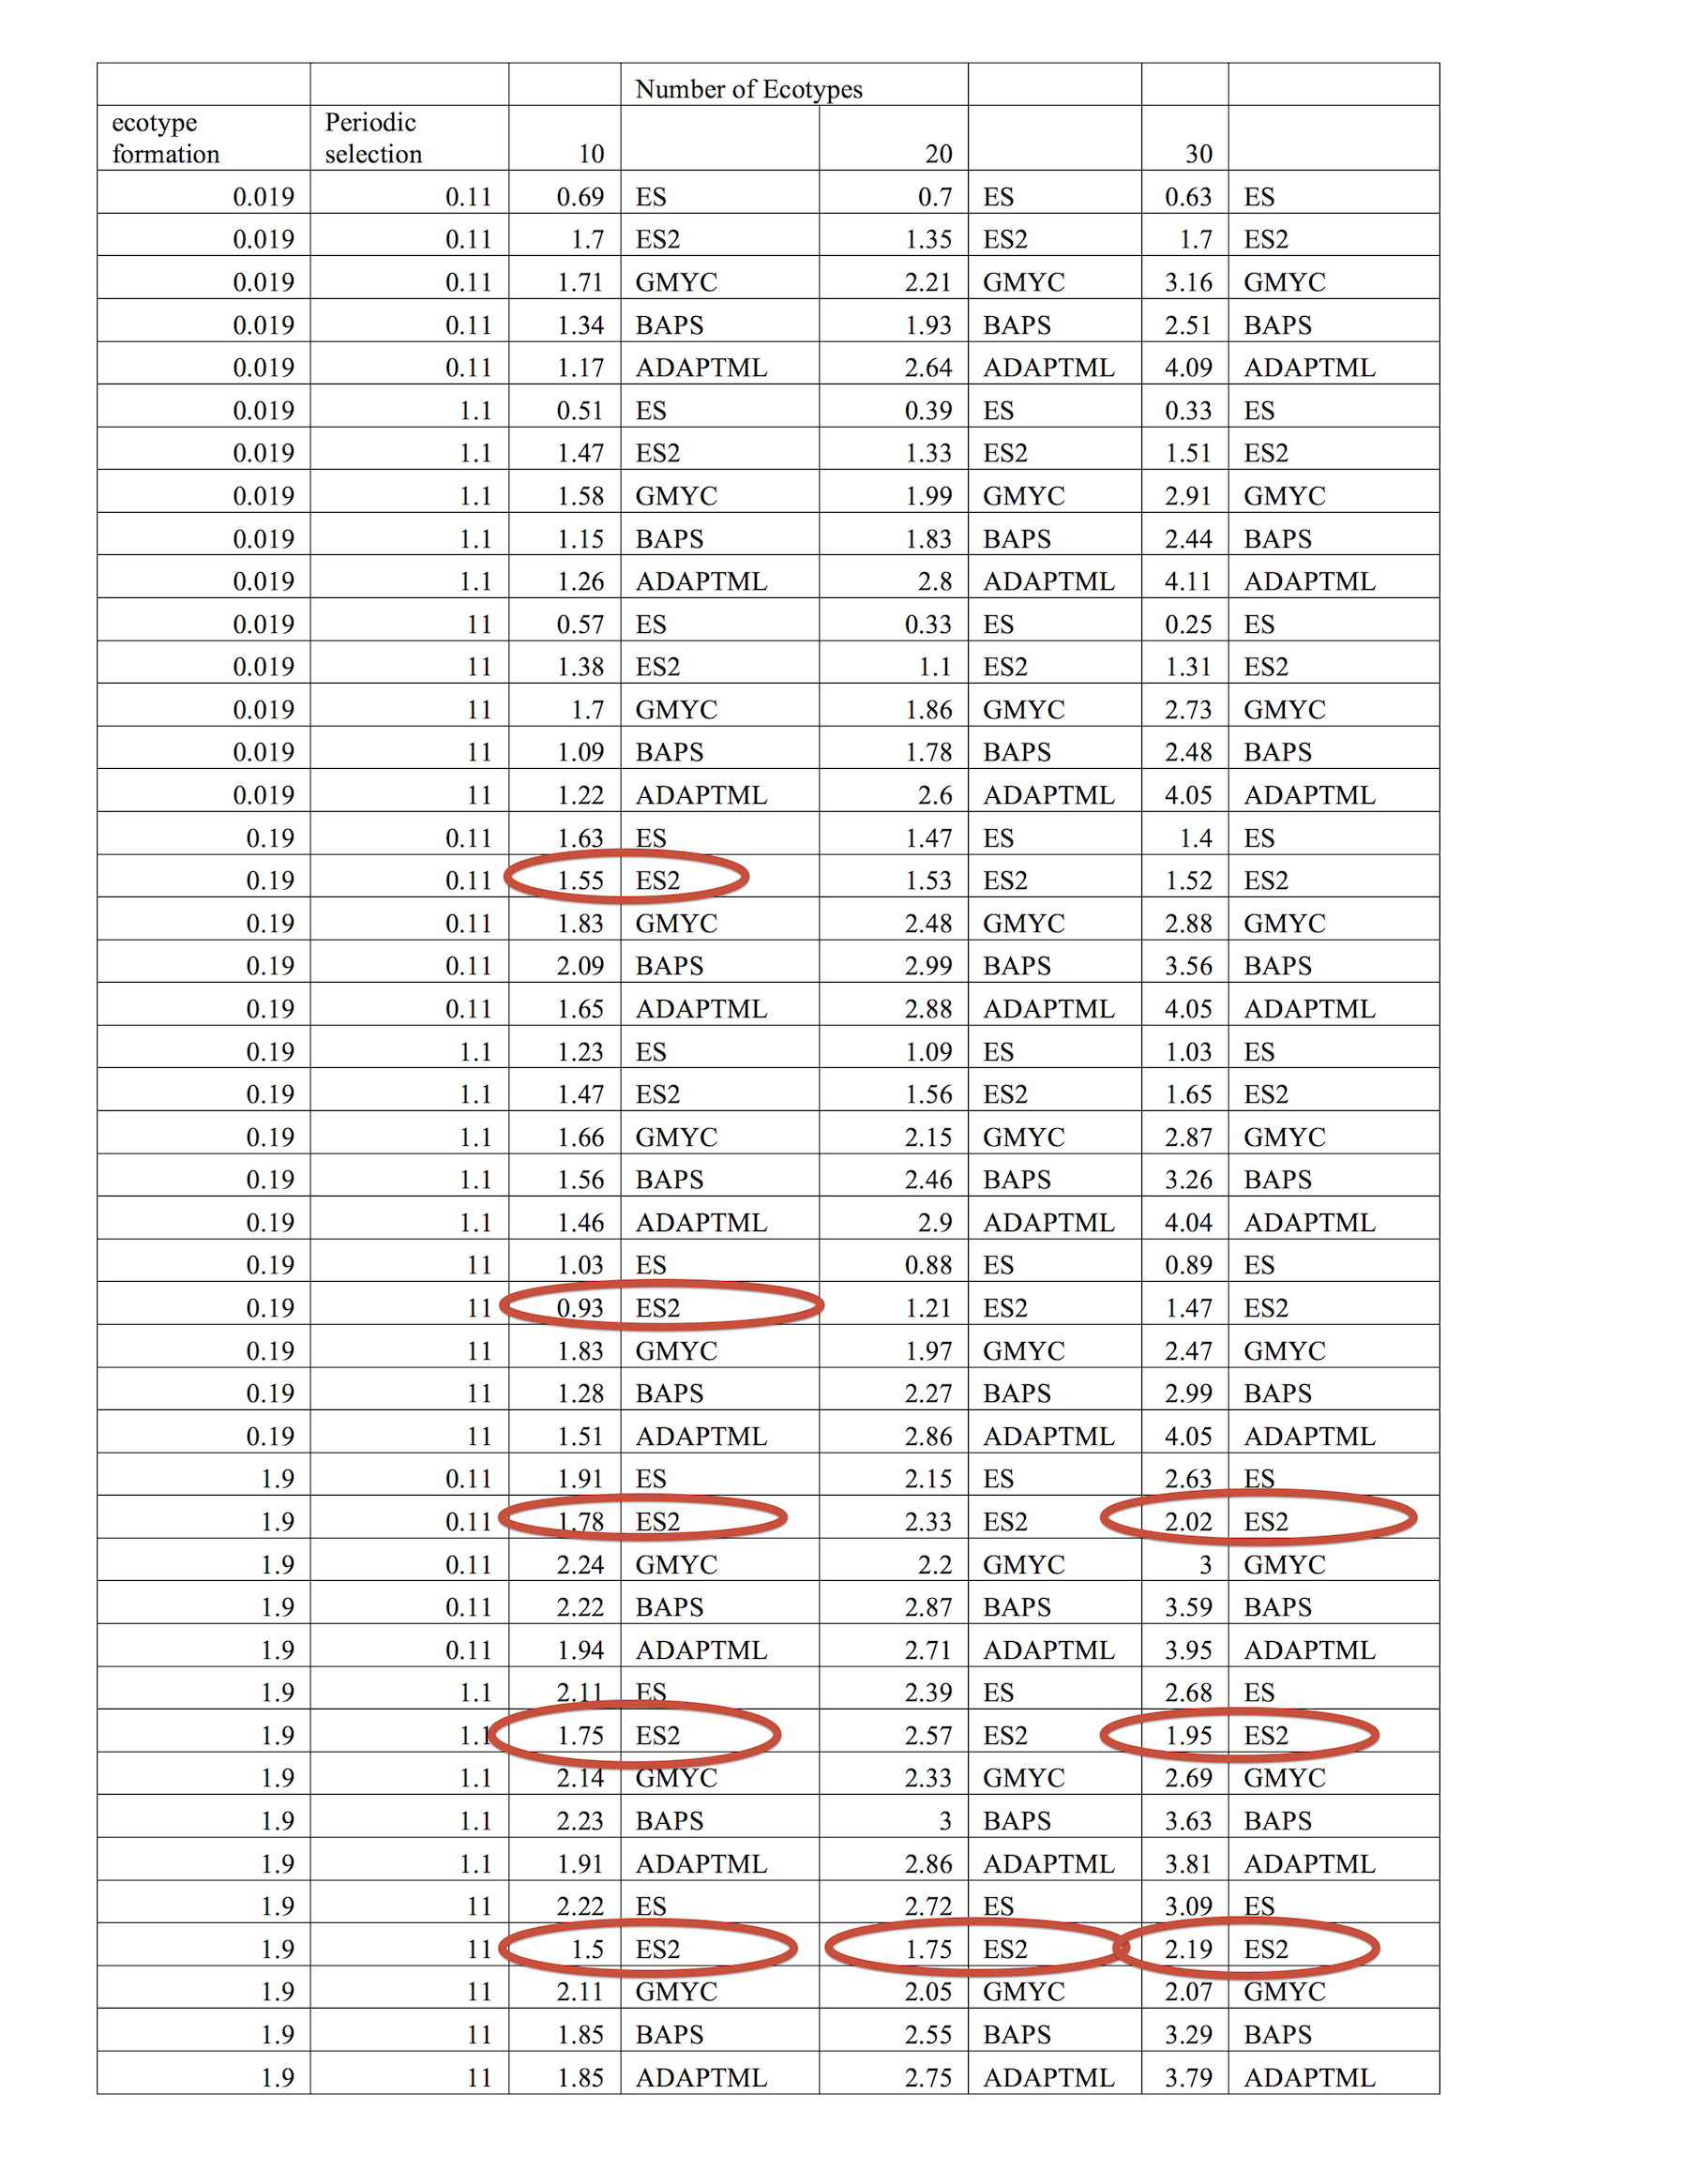
\includegraphics{images/ComparisonTable1.png}
    \label{fig:ComparisonSmall}
\end{figure}

\subsection{Analysis of in silico-generated sequences}
\subsection{\emph{Bacillus} sequences}
\subsection{Running time}